\section{Latent Space optimisation with Weighted Retraining}
\label{sec:lso:main}
\subsection{Training a Generative Model with a Weighted Training Objective}
\label{subsec:weighting}
While it is unclear in general how to design a generative model that is maximally amenable to \gls{lmo},
the argument presented in \cref{sec:lso:limitations} suggests that it would at least be beneficial to dedicate
a higher fraction of the feasible region to modelling high-scoring points.
One obvious but inadequate method of achieving this is to simply discard all low-scoring points from the dataset used to train the \gls{dgm}, e.g.\@ by keeping only the top 10\% of the data set (in terms of score).
While this strategy could be feasible if data is plentiful, when data is scarce this option may not be viable
because state-of-the-art neural networks need a large amount of training data to avoid overfitting.
This issue can be resolved by not viewing inclusion in the dataset as a binary choice,
but instead as a \emph{continuum} that can be realized by \emph{weighting} the data points unevenly.
If the generative model is trained on a distribution that systematically places more probability mass on high-scoring points
and less mass on low-scoring points,
the distribution-matching term in the \gls{dgm}'s training objective will incentivize a larger fraction of the feasible
region's volume to be used to model high-scoring points,
while simultaneously using all known data points to learn useful representations and avoid overfitting.

A simple way to achieve this weighting is to assign an explicit weight $w_i\in[0,1]$ to each data point, such that $\sum_i w_i=1$.
As the training objective of common \glspl{dgm} involves the expected value of a loss
function $\mathcal{L}$ with respect to the data distribution,%
\footnote{For a \gls{vae}, $\mathcal{L}$ is the per-data point ELBO \citep{kingma2013auto}, while for a \gls{gan}, $\mathcal{L}$ is the discriminator score \citep{goodfellow2014generative}.}
weighted training can be implemented by simply replacing the empirical mean over the training data with a \emph{weighted} empirical mean:
i.e.\@ $\sum_{\x_i \in \D} w_i\mathcal{L}(\x_i)$ instead of $\sum_{\x_i \in \D} \frac{1}{N} \mathcal{L}(\x_i)$.
In practice, mini-batch stochastic gradient descent is used to optimise this objective
to avoid summing over all data points.
Unbiased mini-batches can be constructed by sampling each data point $\x_i$ with probability $w_i$
with replacement to construct each batch.

We offer no universal rules for setting weights, except that all weights $w_i$ should be restricted to strictly positive values,
because a negative weight would incentivize the model to perform poorly,
and a weight of zero is equivalent to discarding a point.
This aside, there are many reasonable ways to choose the weights such that high-scoring points are weighted more,
and low-scoring points are weighted less.
In this work, we decide to use a rank-based weight function,
\begin{equation}
\label{eq:weighting_function}
    w(\x; \D, k) \propto \frac{1}{kN + \text{rank}_{f,\D}(\x)}, \quad \text{rank}_{f,\D}(\x) = \left|\left\{\x_i : f(\x_i) > f(\x),\ \x_i \in \D \right\}\right|\ ,
\end{equation}
which assigns a weight roughly proportional to the reciprocal (zero-based) rank of each data point.
We chose \cref{eq:weighting_function} because it yields weights which are always positive,
resilient to outliers by virtue of using ranks, and will behave similarly over a range of dataset sizes.
Furthermore, as shown in \cref{fig:weighting}, it admits a single tunable hyperparameter $k\in(0,\infty)$ which continuously controls the degree of weighting,
where $k\to\infty$ corresponds to uniform weighting, i.e.\@ $w_i = \frac{1}{N}, \forall i$, while $k\to0$ places \emph{all} mass on only the single point with the highest objective function value.

\begin{figure}[ht]
    \centering
    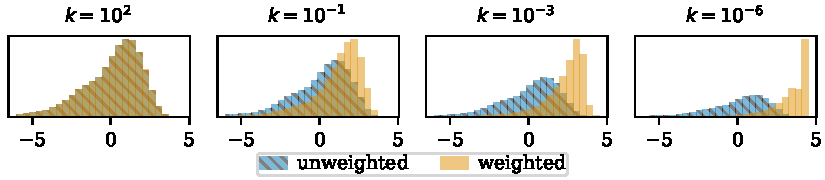
\includegraphics{histograms/train-data-hist-chem.pdf}
    \caption[Histogram of objective function values for the ZINC dataset]{
    Histogram of objective function values for the ZINC dataset (see \cref{sec:lso:experiments})
    with uniform weighting (in blue) as well as rank weighting from \cref{eq:weighting_function} for different $k$ values (in orange).
    Large $k$ approaches uniform weighting, while small $k$ places most weight on high-scoring points.
    }
    \label{fig:weighting}
\end{figure}

\subsection{Periodic Retraining to Update the Latent Space}
\label{subsec:retraining}
To allow the latent manifold to adapt to new information,
we propose a conceptually simple solution: \emph{periodically retraining the generative model} during the optimisation procedure.
In practice, this could be done by training a new model from scratch,
or by fine-tuning the previously trained model on the novel data.
However, as is often pointed out in the active learning literature,
the effect of adding a few additional points to a large dataset is rather negligible,
and thus it is unlikely that the generative model will change significantly if retrained on
this augmented dataset \citep{sener_active_2018}.
While one could also retrain on \emph{only} the new data,
this might lead to the well-known phenomenon of catastrophic forgetting \citep{mccloskey_catastrophic_1989}.

A key observation we make is that \emph{the data weighting outlined in \cref{subsec:weighting} actually resolves this problem}.
Specifically, if the new points queried are high-scoring,
then a suitable weighting scheme (such as \cref{eq:weighting_function}) will assign a large weight to them,
while simultaneously decreasing the weights of many of the original data points,
meaning that a small number of new points can have a disproportionate impact on the training distribution.
If the generative model is then retrained using this distribution,
it can be expected to change significantly to incorporate these new points into the latent space in order to minimise the weighted loss.
By contrast, if the new points queried are low-scoring,
then the distribution will change negligibly, and the generative model will not significantly update, thereby avoiding adding new low-scoring points into the feasible region.
\subsection{Weighted Retraining Combined}
\label{subsec:weighted-retraining}
When put together, \emph{data weighting} and \emph{periodic retraining} complement each other elegantly,
transforming the generative model from a passive decoding function into an active participant
in the optimisation process,
whose role is to ensure that the latent manifold is constantly
occupied by the most updated and relevant points for optimisation.
Their combined effect is visualized conceptually in \cref{subfig:lso-schematic-c}.
In the first iteration, weighted training creates a latent space with more high scoring points,
causing the feasible region to extend farther into the green region at the expense of the red region.
This allows a better orange point to be chosen relative to \cref{subfig:lso-schematic-b}.
In the second iteration in \cref{subfig:lso-schematic-c},
weighted training with the orange point 
incorporates even more high-scoring points into the latent space,
allowing an even better point to be found.
Qualitatively similar results can be seen in the 2D shape area maximisation task,
where weighted retraining introduces points with very high areas
into the latent space compared to \cref{subfig:lso-schematic-a}
(details for this experiment are given in \cref{sec:lso:experiments}).

\begin{algorithm}[tb]
\caption{Latent Space optimisation {\color{blue} with Weighted Retraining} (changes highlighted in {\color{blue} blue}).}
\label{alg:lso-weighted-retraining}
\begin{algorithmic}[1]
    \STATE {\bfseries Input:} Data $\D = \{(\x_i, f(\x_i))\}_{i=1}^N$, query budget $M$, objective function $f(\x)$, latent objective model $\hat f(\z)$,
    generative/inverse model $g(\z)$/$q(\x)$, {\color{blue} retrain frequency $r$, weighting function $w(\x)$}
    \vspace{1mm}
    {\color{blue}\FOR{$1, \ldots, M$\textcolor{blue}{$/r$}}
        {\color{black} \STATE Train generative model $g$ and inverse model $q$ on data $\D$ {\color{blue} weighted by $\mathcal{W} = \{w(\x)\}_{\x \in \D}$}%
        \vspace{1mm}
    	\FOR{$1, \ldots, $\textcolor{blue}{$r$}}
            \STATE Compute latent variables $\mathcal{Z} = \{\z = q(\x)\}_{\x \in \D}$
            \STATE Fit objective model $\hat f$ to $\mathcal{Z}$ and $\D$,
            and optimise $\hat f$
            to obtain new latent query point $\tilde{\z}$
    	    \STATE Obtain corresponding input $\tilde{\x} = g(\tilde{\z})$, evaluate $f(\tilde{\x})$ and set $\D \gets \D \cup \{(\tilde{\x}, f(\tilde{\x}))\}$
        \ENDFOR}
    \ENDFOR}
    \vspace{1mm}
	\STATE {\bfseries Output:} Augmented dataset $\D$
\end{algorithmic} 
\end{algorithm}

In the remainder of this chapter, we refer to the combination of these techniques as
\emph{weighted retraining} for brevity; see \cref{alg:lso-weighted-retraining} for pseudocode.
Computationally, the overhead of the weighting is minimal, and the cost of the retraining
can be reduced by fine-tuning an existing model on the weighted dataset instead of retraining it from scratch.
Although this may still be prohibitively expensive for some applications,
we stress that in many scenarios the cost of training a model is insignificant compared to even a single evaluation of the objective function (e.g.\@ performing wet-lab experiments for drug design),
making weighted retraining a sensible choice.
